% PDF
\documentclass{beamer}
\usepackage{tikz}

\usetikzlibrary{math,calc,shadows}

\title{Git}

\mode<presentation>
\usetheme[height=.75cm,compress]{Singapore}
\setbeamertemplate{title page}{%
  \begin{center}
    {\sc Projectweek} \\
    \rule[10pt]{5cm}{1pt} \\
    {\sc\Huge \inserttitle}
  \end{center}
}

\setbeamertemplate{navigation symbols}{}

\makeatletter

\tikzset{
    git/.cd,
    commit/.style={draw,circle,minimum size=0.2cm},
    commit arrow/.style={thick,-latex},
    ref/.style={draw,fill=blue!50,font=\tiny\ttfamily},
    head/.style={git/ref,fill=red!50},
}

\tikzset{
    fs/.cd,
    directory/.style={font=\ttfamily},
    dirlink/.style={thick},
}

\tikzset{
  console/.style={fill=black,text=green!50,font=\ttfamily\small},
  comment box/.style={fill=blue!25,opacity=0.9,text opacity=1,overlay,text=black},
  comment line/.style={blue,thick,overlay},
  copy arrow/.style={green!50!black,thick,-latex},
  move arrow/.style={green!50!black,thick,-latex},
}


\pgfkeys{
  /fs/directory/.cd,
  id/.initial=dir,
  id/.value required,
  position/.initial={(0,0)},
  position/.value required,
  subdirectory of/.code args={#1 distance #2}{\pgfkeysalso{/fs/directory/position={($ (#1) + (0.4,#2 * -0.5) $)}}}
}

\newcommand{\directory}[2][]{{
  \pgfkeys{
    /fs/directory/.cd,
    #1,
    /fs/directory/id/.get=\dirid,
    /fs/directory/position/.get=\dirpos,
  }
  \draw[fill] \dirpos coordinate (\dirid) circle[radius=0.05cm] node[anchor=west,fs/directory] (\dirid-node) {#2};
}}

\pgfkeys{
  /codeline/.cd,
  x/.initial=0,
  y/.initial=0,
  color/.initial=black,
}

\newcommand{\codeline}[1][]{{
  \pgfkeys{
    /codeline/.cd,
    #1,
    /codeline/x/.get=\codeline@xcoordinate,
    /codeline/y/.get=\codeline@ycoordinate,
    /codeline/color/.get=\codeline@color,
  }
  \tikzmath{
    real \codeline@width;
    real \codeline@y;
    \codeline@y=abs(\codeline@ycoordinate);
    \codeline@width=mod(\codeline@y*521.2+\codeline@y*\codeline@y*15.4+0.5,3)+0.2;
  }
  \draw[thick,\codeline@color] (\codeline@xcoordinate,\codeline@ycoordinate) -- ++(\codeline@width,0);
}}

\newcommand{\master}{master}

\makeatother

\begin{document}

\begin{frame}[plain]
  \titlepage
\end{frame}

% IGNORE

\section{Version Control}

\begin{frame}
  \tableofcontents[currentsection]
\end{frame}

\begin{frame}
  \frametitle{Problem Statement}
  \begin{itemize}
    \item Modifying code is risky
    \item We might break something
    \item Keep a fully functional version somewhere safe (= a backup)
    \item In case of trouble, we can simply restore this backup
  \end{itemize}
\end{frame}

\begin{frame}
  \frametitle{Manual Solution}
  \begin{center}
    \begin{tikzpicture}
      \path[use as bounding box] (0,0) rectangle (3,-3);
      \directory[id=root,position={(0,0)}]{project}
      \directory[id=working-area,subdirectory of=root distance 1]{working-area}
      \directory[id=wa-src,subdirectory of=working-area distance 1]{src}
      \directory[id=wa-app,subdirectory of=wa-src distance 1]{app.py}
      \directory[id=wa-lib,subdirectory of=wa-src distance 2]{lib.py}
      \directory[id=backup,subdirectory of=root distance 5]{backup}

      \only<3->{
        \directory[id=bu-src,subdirectory of=backup distance 1]{src}
        \directory[id=bu-app,subdirectory of=bu-src distance 1]{app.py}
        \directory[id=bu-lib,subdirectory of=bu-src distance 2]{lib.py}
      }

      \draw[fs/dirlink] (root) |- (backup);
      \draw[fs/dirlink] (root) |- (working-area);
      \draw[fs/dirlink] (working-area) |- (wa-src);
      \draw[fs/dirlink] (wa-src) |- (wa-app);
      \draw[fs/dirlink] (wa-src) |- (wa-lib);

      \only<3->{
        \draw[fs/dirlink] (backup) |- (bu-src);
        \draw[fs/dirlink] (bu-src) |- (bu-app);
        \draw[fs/dirlink] (bu-src) |- (bu-lib);
      }

      \only<1>{
        \draw[comment line,latex-] (working-area-node.east) -| ++(1,0.75) node[comment box,anchor=south] (comment) {Develop code in this folder};
      }
      \only<2>{
        \draw[comment line,latex-] (backup-node.east) -| ++(2,-0.5) node[comment box,anchor=north] {Regularly copy code into here};
      }
      \only<3>{
        \draw[copy arrow] (working-area-node.east) -- ++(1,0) |- (backup-node.east) node[midway,below] {copy};
      }
    \end{tikzpicture}
  \end{center}
  \vskip1cm
  \begin{overprint}
    \onslide<3>
    \begin{center}
      
\begin{tikzpicture}
        \node[console] {
          \parbox{8cm}{
            \# Inside working-area \\
            \$ rm -r ../backup \\
            \$ cp -r * ../backup
          }
        };
      \end{tikzpicture}
    \end{center}
  \end{overprint}
\end{frame}

\begin{frame}
  \frametitle{Problem Statement}
  \begin{itemize}
    \item We don't just want backup of last working version
    \item We'd like to keep track of \emph{all} previous versions
    \item We need a separate directory per backup
  \end{itemize}
\end{frame}

\begin{frame}
  \frametitle{Manual Solution}
  \begin{center}
    \begin{tikzpicture}
      \path[use as bounding box] (0,0) rectangle (3,-2);
      \directory[id=root,position={(0,0)}]{project}
      \directory[id=working-area,subdirectory of=root distance 1]{working-area}
      \directory[id=backups,subdirectory of=root distance 2]{backups}

      \draw[fs/dirlink] (root) |- (backups);
      \draw[fs/dirlink] (root) |- (working-area);

      \only<2->{
        \directory[id=backup1,subdirectory of=backups distance 1]{20220329-1531}
        \draw[fs/dirlink] (backups) |- (backup1);
      }

      \only<2>{
        \draw[copy arrow] (working-area-node.east) -- ++(1,0) |- (backup1-node.east);
      }

      \only<3->{
        \directory[id=backup2,subdirectory of=backups distance 2]{20220330-1022}
        \draw[fs/dirlink] (backups) |- (backup2);
      }

      \only<3>{
        \draw[copy arrow] (working-area-node.east) -- ++(1,0) |- (backup2-node.east);
      }

      \only<4->{
        \directory[id=backup3,subdirectory of=backups distance 3]{20220331-1503}
        \draw[fs/dirlink] (backups) |- (backup3);
      }

      \only<4>{
        \draw[copy arrow] (working-area-node.east) -- ++(1,0) |- (backup3-node.east);
      }

    \end{tikzpicture}
  \end{center}
  \vskip1cm
  \begin{overprint}
    \onslide<2-4>
    \begin{center}
      
\begin{tikzpicture}
        \node[console] {
          \parbox{8cm}{
            \# Inside working-area \\
            \$ DIR=../backups/\`{}date +\%Y\%m\%d-\%H\%m\`{} \\
            \$ mkdir -p \$DIR \\
            \$ cp -r * \$DIR
          }
        };
      \end{tikzpicture}
    \end{center}
  \end{overprint}
\end{frame}

\begin{frame}
  \frametitle{Git To The Rescue}
  \begin{itemize}
    \item Git automates this process
    \item Git is smart about storage
      \begin{itemize}
        \item Will not duplicate files needlessly
        \item Uses delta compression
      \end{itemize}
  \end{itemize}
\end{frame}

\begin{frame}
  \frametitle{Git Modus Operandi}
  \begin{center}
    \begin{tikzpicture}
      \directory[id=root,position={(0,0)}]{project}
      \directory[id=git,subdirectory of=root distance 1]{.git}
      \directory[id=src,subdirectory of=root distance 2]{src}
      \directory[id=app,subdirectory of=src distance 1]{app.py}
      \directory[id=lib,subdirectory of=src distance 2]{lib.py}

      \draw[fs/dirlink] (root) |- (git);
      \draw[fs/dirlink] (root) |- (src);
      \draw[fs/dirlink] (src) |- (app);
      \draw[fs/dirlink] (src) |- (lib);

      \visible<4->{
        \node[git/commit] (commit v1) at (0,-3) {v1};
      }
      \visible<7->{
        \node[git/commit] (commit v2) at ($ (commit v1) + (2,0) $) {v2};
        \draw[git/commit arrow] (commit v1) -- (commit v2);
      }

      \begin{scope}[overlay]
        \only<1>{
          \draw[comment line,latex-] (root-node.east) -| ++(1,0.5) node[comment box,anchor=south] {You work directly in project's root directory};
        }
        \only<2>{
          \draw[comment line,latex-] (git-node.east) -| ++(1,1) node[comment box,anchor=south] {Git stores data in hidden directory};
        }
        \only<3>{
          \draw[comment line,latex-] (app-node.east) -| ++(1,-1) node[comment box,anchor=north] (explanation) {\parbox{5cm}{First, you must let Git know which files should be backed up}};
          \draw[comment line,latex-] (lib-node.east) -| (explanation.north);
        }
        \only<4>{
          \draw[comment line,latex-] (git-node.east) -| ++(1.5,0.75) node[comment box,anchor=south] {\parbox{5cm}{\emph{Committing} tells Git to take a snapshot and store it internally}};
          \draw[comment line,latex-] (commit v1.west) -| ++(-1.25,0.75) node[comment box,anchor=south] {\parbox{3cm}{We represent a commit by a circle}};
        }
        \only<5>{
          \draw[comment line,latex-] (app-node.east) -| ++(1,-1) node[comment box,anchor=north] (explanation) {Say you update this file};
        }
        \only<6>{
          \draw[comment line,latex-] (app-node.east) -| ++(1,-1) node[comment box,anchor=north] (explanation) {\parbox{5cm}{We need to tell Git explicitly which file changes to commit}};
        }
        \only<7>{
          \draw[comment line,latex-] (commit v2.east) -| ++(1,-0.5) node[comment box,anchor=north] {A new commit is added};
        }
      \end{scope}
    \end{tikzpicture}
  \end{center}
  \vskip1cm
  \begin{overprint}
    \onslide<3>
    \begin{center}
      
\begin{tikzpicture}
        \node[console] {
          \parbox{8cm}{
            \$ git add src/*.py
          }
        };
      \end{tikzpicture}
    \end{center}

    \onslide<4>
    \begin{center}
      
\begin{tikzpicture}
        \node[console] {
          \parbox{8cm}{
            \$ git commit -m 'v1'
          }
        };
      \end{tikzpicture}
    \end{center}

    \onslide<6>
    \begin{center}
      
\begin{tikzpicture}
        \node[console] {
          \parbox{8cm}{
            \$ git add src/app.py
          }
        };
      \end{tikzpicture}
    \end{center}

    \onslide<7>
    \begin{center}
      
\begin{tikzpicture}
        \node[console] {
          \parbox{8cm}{
            \$ git commit -m 'v2'
          }
        };
      \end{tikzpicture}
    \end{center}
  \end{overprint}
\end{frame}

\begin{frame}
  \frametitle{Commit Chain}
  \begin{center}
    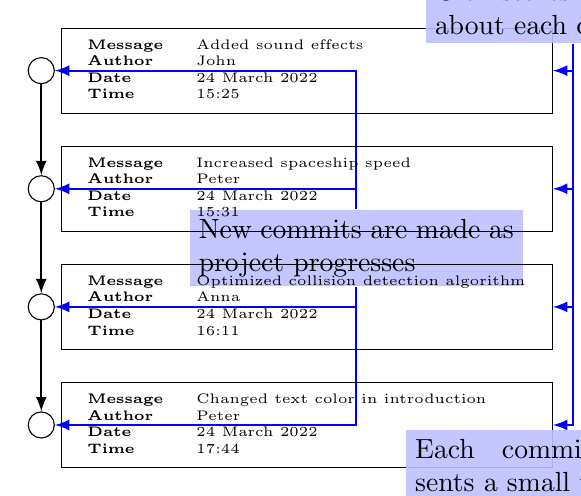
\begin{tikzpicture}[commit data/.style={draw}]
      \foreach[evaluate={-1.5*(\i-1)} as \y] \i in {1,...,4} {
        \coordinate (commit position \i) at (0,\y);
      }

      \node[git/commit] (commit 1) at (commit position 1) {};

      \visible<1-4>{
        \node[comment box,overlay] (comment) at ($ (commit position 1) ! 0.5 ! (commit position 4) + (4,0) $) {\parbox{4cm}{New commits are made as project progresses}};
      }
      \visible<1>{
        \draw[comment line,latex-,overlay] (commit 1.east) -| (comment);
      }

      \foreach[evaluate={int(\i-1)} as \j,evaluate={\i} as \slideindex] \i in {2,...,4} {
        \visible<\slideindex->{
          \node[git/commit] (commit \i) at (commit position \i) {};
          \draw[git/commit arrow] (commit \j) -- (commit \i);
        }
        \visible<\slideindex>{
          \draw[comment line,latex-] (commit \i.east) -| (comment);
        }
      }

      \visible<5->{
        \node[anchor=west,font=\tiny,commit data] (commit data 1) at ($ (commit 1) + (0.25,0) $) {
          \parbox{6cm}{
            \begin{tabular}{ll}
              \textbf{Message} & Added sound effects \\
              \textbf{Author} & John \\
              \textbf{Date} & 24 March 2022 \\
              \textbf{Time} & 15:25 \\
            \end{tabular}
          }
        };

        \node[anchor=west,font=\tiny,commit data] (commit data 2) at ($ (commit 2) + (0.25,0) $) {
          \parbox{6cm}{
            \begin{tabular}{ll}
              \textbf{Message} & Increased spaceship speed \\
              \textbf{Author} & Peter \\
              \textbf{Date} & 24 March 2022 \\
              \textbf{Time} & 15:31 \\
            \end{tabular}
          }
        };

        \node[anchor=west,font=\tiny,commit data] (commit data 3) at ($ (commit 3) + (0.25,0) $) {
          \parbox{6cm}{
            \begin{tabular}{ll}
              \textbf{Message} & Optimized collision detection algorithm \\
              \textbf{Author} & Anna \\
              \textbf{Date} & 24 March 2022 \\
              \textbf{Time} & 16:11 \\
            \end{tabular}
          }
        };

        \node[anchor=west,font=\tiny,commit data] (commit data 4) at ($ (commit 4) + (0.25,0) $) {
          \parbox{6cm}{
            \begin{tabular}{ll}
              \textbf{Message} & Changed text color in introduction \\
              \textbf{Author} & Peter \\
              \textbf{Date} & 24 March 2022 \\
              \textbf{Time} & 17:44 \\
            \end{tabular}
          }
        };
      }

      \visible<5>{
        \begin{scope}[overlay]
          \node[comment box] (comment) at ($ (commit data 1.north east) + (0.25,0.25) $) {\parbox{3.5cm}{Git stores metadata about each commit}};
          \draw[comment line,-latex] (comment.south) |- (commit data 1.east);
          \draw[comment line,-latex] (comment.south) |- (commit data 2.east);
          \draw[comment line,-latex] (comment.south) |- (commit data 3.east);
          \draw[comment line,-latex] (comment.south) |- (commit data 4.east);
        \end{scope}
      }

      \visible<6>{
        \node[comment box] at ($ (commit data 4.south east) $) {\parbox{3.5cm}{Each commit represents a small update}};
      }
    \end{tikzpicture}
  \end{center}
\end{frame}

% IGNORE

\section{Branching}

\begin{frame}
  \tableofcontents[currentsection]
\end{frame}

\begin{frame}
  \frametitle{Problem Statement}
  \begin{itemize}
    \item Developing a new feature can take a lot of work
    \item Multiple teams work on different features in parallel
    \item Teams do not want to interfere with each other
  \end{itemize}
\end{frame}

\begin{frame}
  \frametitle{Manual Solution}
  \begin{center}
    \begin{tikzpicture}
      \path[use as bounding box] (0,0) rectangle ++(6,-6.5);
      \directory[id=root,position={(0,0)}]{project}
      \directory[id=trunk,subdirectory of=root distance 1]{trunk}
      \directory[id=tb1,subdirectory of=trunk distance 1]{20220329-1531}
      \directory[id=tb2,subdirectory of=trunk distance 2]{20220330-1022}
      \directory[id=tb3,subdirectory of=trunk distance 3]{20220330-1357}

      \only<3->{
        \directory[id=feature a,subdirectory of=root distance 5]{feature-a}
        \directory[id=a working area,subdirectory of=feature a distance 1]{working-area}
      }

      \only<5->{
        \directory[id=a backups,subdirectory of=feature a distance 2]{backups}
        \directory[id=a backups 1,subdirectory of=a backups distance 1]{20220331-1403}
      }

      \only<6->{
        \directory[id=feature b,subdirectory of=root distance 9]{feature-b}
        \directory[id=b working area,subdirectory of=feature b distance 1]{working-area}
        \directory[id=b backups,subdirectory of=feature b distance 2]{backups}
        \directory[id=b backups 1,subdirectory of=b backups distance 1]{20220331-1611}
      }

      \draw[fs/dirlink] (root) |- (trunk);
      \draw[fs/dirlink] (trunk) |- (tb1);
      \draw[fs/dirlink] (trunk) |- (tb2);
      \draw[fs/dirlink] (trunk) |- (tb3);

      \only<3->{
        \draw[fs/dirlink] (root) |- (feature a);
        \draw[fs/dirlink] (feature a) |- (a working area);
      }
      \only<5->{
        \draw[fs/dirlink] (feature a) |- (a backups);
        \draw[fs/dirlink] (a backups) |- (a backups 1);
      }

      \only<6->{
        \draw[fs/dirlink] (root) |- (feature b);
        \draw[fs/dirlink] (feature b) |- (b working area);
        \draw[fs/dirlink] (feature b) |- (b backups);
        \draw[fs/dirlink] (b backups) |- (b backups 1);
      }

      \only<1>{
        \draw[comment line,latex-] (trunk-node.east) -- ++(0.5,0) |- ++(2,0.25) node[comment box,anchor=west] (comment) {\parbox{4cm}{Contains all versions of the project}};
        \draw[comment line,latex-] (tb1-node.east) -| (comment);
        \draw[comment line,latex-] (tb2-node.east) -| (comment);
        \draw[comment line,latex-] (tb3-node.east) -| (comment);
      }

      \only<2>{
        \draw ($ (trunk-node.east) + (2.5,0.25) $) node[comment box,anchor=west] {\parbox{4cm}{Say we wish to develop some new feature A}};
      }

      \only<3>{
        \draw[comment line,latex-] (trunk-node.east) -- ++(0.5,0) |- ++(2,0.25) node[comment box,anchor=west] {\parbox{4cm}{We do not develop directly on \texttt{trunk}}};
        \draw[comment line,latex-] (a working area-node.south) -- ++(0,-1) node[comment box,anchor=north] {\parbox{4cm}{Instead, we copy the latest version to a separate directory}};
        \draw[copy arrow] (tb3-node.east) -- ++(0.2,0) |- (a working area-node.east);
      }

      \only<4>{
        \draw[comment line,latex-] (a working area-node.south) -- ++(0,-1) node[comment box,anchor=north] {\parbox{4cm}{We develop feature A in this separate directory}};
      }

      \only<5>{
        \draw[comment line,latex-] (a backups 1-node.south) -- ++(0,-1) node[comment box,anchor=north] {We regularly make backups};
        \draw[copy arrow] (a working area-node.east) -- ++(1,0) |- (a backups 1-node.east);
      }

      \only<6>{
        \draw[comment line,latex-] (feature b-node.east) -- ++(2,0) node[comment box,anchor=west] (comment) {\parbox{4cm}{A different feature can be developed in parallel by another team in a separate directory}};
      }
    \end{tikzpicture}
  \end{center}
\end{frame}

\begin{frame}
  \frametitle{Git Branches}
  \begin{center}
    \begin{tikzpicture}
      \node[git/commit] (commit 1) at (0,0) {};
      \node[git/commit] (commit 2) at ($ (commit 1) + (1,0) $) {};
      \node[git/commit] (commit 3) at ($ (commit 2) + (1,0) $) {};
      \node[git/commit] (commit 4) at ($ (commit 3) + (1,0) $) {};

      \visible<5->{
        \node[git/commit] (a commit 1) at ($ (commit 4) + (1,1) $) {};
      }
      \visible<6->{
        \node[git/commit] (a commit 2) at ($ (a commit 1) + (1,0) $) {};
      }
      \visible<7->{
        \node[git/commit] (a commit 3) at ($ (a commit 2) + (1,0) $) {};
      }

      \visible<8->{
        \node[git/commit] (b commit 1) at ($ (commit 4) + (1,-1) $) {};
        \node[git/commit] (b commit 2) at ($ (b commit 1) + (1,0) $) {};
      }

      \draw[git/commit arrow] (commit 1) -- (commit 2);
      \draw[git/commit arrow] (commit 2) -- (commit 3);
      \draw[git/commit arrow] (commit 3) -- (commit 4);

      \visible<5->{
        \draw[git/commit arrow] (commit 4) -- (a commit 1);
      }
      \visible<6->{
        \draw[git/commit arrow] (a commit 1) -- (a commit 2);
      }
      \visible<7->{
        \draw[git/commit arrow] (a commit 2) -- (a commit 3);
      }

      \visible<8->{
        \draw[git/commit arrow] (commit 4) -- (b commit 1);
        \draw[git/commit arrow] (b commit 1) -- (b commit 2);
      }

      \visible<3->{
        \draw[latex-] (commit 4) -- ++(0,-1) node[git/ref] (master) { \master };
      }
      \visible<4>{
        \draw[latex-] (commit 4) -- ++(0,1) node[git/ref] (feature a) { feature-a };
      }
      \visible<5>{
        \draw[latex-] (a commit 1) -- ++(0,1) node[git/ref] (feature a 1) { feature-a };
      }
      \visible<6>{
        \draw[latex-] (a commit 2) -- ++(0,1) node[git/ref] (feature a 2) { feature-a };
      }
      \visible<7-8>{
        \draw[latex-] (a commit 3) -- ++(0,1) node[git/ref] (feature a 3) { feature-a };
      }
      \visible<8>{
        \draw[latex-] (b commit 2) -- ++(0,-1) node[git/ref] (feature b 2) { feature-b };
      }

      \only<1>{
        \begin{scope}[overlay]
          \node[anchor=south,comment box] (comment) at ($ (commit 1) ! 0.5 ! (commit 4) + (0,1) $) {These are the \texttt{trunk} commits};
          \draw[comment line,-latex] (comment) -- (commit 1);
          \draw[comment line,-latex] (comment) -- (commit 2);
          \draw[comment line,-latex] (comment) -- (commit 3);
          \draw[comment line,-latex] (comment) -- (commit 4);
        \end{scope}
      }

      \only<2>{
        \begin{scope}[overlay]
          \draw[comment line,latex-] (commit 4) -- ++(0,-1) node[comment box,anchor=north] {Git calls this the "\texttt{master} branch"};
        \end{scope}
      }

      \only<3>{
        \begin{scope}[overlay]
          \draw[comment line,latex-] (master) -- ++(0,-1) node[comment box,anchor=north] {\parbox{6cm}{Git labels the most recent commit with the name of the branch}};
        \end{scope}
      }

      \only<4>{
        \begin{scope}[overlay]
          \draw[comment line,latex-] (feature a) -- ++(0,1) node[comment box,anchor=south] {We can create a new branch};
        \end{scope}
      }

      \only<5>{
        \begin{scope}[overlay]
          \draw[comment line,latex-] (a commit 1) -- ++(-0.75,0.5) node[comment box,anchor=south east] {\parbox{5cm}{We can make commits on this new branch}};
          \draw[comment line,latex-] (master) -- ++(0,-0.5) node[comment box,anchor=north] {\texttt{\master} still exists at same location};
        \end{scope}
      }

      \only<8>{
        \begin{scope}[overlay]
          \draw[comment line,latex-] (feature b 2) -- ++(0,-0.5) node[comment box,anchor=north] {\parbox{4.5cm}{We can create as many branches as we wish}};
        \end{scope}
      }
    \end{tikzpicture}
  \end{center}
  \vskip1cm
  \begin{overprint}
    \onslide<4>
    \begin{center}
      
\begin{tikzpicture}
        \node[console] {
          \$ git branch feature-a
        };
      \end{tikzpicture}
    \end{center}

    \onslide<5>
    \begin{center}
      
\begin{tikzpicture}
        \node[console] {
          \$ git commit -m "did something for feature a"
        };
      \end{tikzpicture}
    \end{center}

    \onslide<6>
    \begin{center}
      
\begin{tikzpicture}
        \node[console] {
          \$ git commit -m "did some more"
        };
      \end{tikzpicture}
    \end{center}

    \onslide<7>
    \begin{center}
      
\begin{tikzpicture}
        \node[console] {
          \$ git commit -m "another addition to feature a"
        };
      \end{tikzpicture}
    \end{center}
  \end{overprint}
\end{frame}

\begin{frame}
  \frametitle{Git Branches on Disk}
  \begin{center}
    \begin{tikzpicture}
      \directory[id=root,position={(0,0)}]{project}
      \directory[id=git,subdirectory of=root distance 1]{.git}
      \directory[id=src,subdirectory of=root distance 2]{src}
      \directory[id=app,subdirectory of=src distance 1]{app.py}

      \draw[fs/dirlink] (root) |- (git);
      \draw[fs/dirlink] (root) |- (src);
      \draw[fs/dirlink] (src) |- (app);

      \begin{scope}[xshift=6cm,yshift=1cm]
        \node[git/commit] (commit 1) at (0,0) {};
        \node[git/commit] (commit 2) at ($ (commit 1) + (0,-1) $) {};
        \node[git/commit] (commit 3) at ($ (commit 2) + (0,-1) $) {};
        \node[git/commit] (a commit 1) at ($ (commit 3) + (-0.5,-1) $) {};
        \node[git/commit] (a commit 2) at ($ (a commit 1) + (0,-1) $) {};
        \node[git/commit] (a commit 3) at ($ (a commit 2) + (0,-1) $) {};
        \node[git/commit] (b commit 1) at ($ (commit 3) + (0.5,-1) $) {};
        \node[git/commit] (b commit 2) at ($ (b commit 1) + (0,-1) $) {};

        \draw[git/commit arrow] (commit 1) -- (commit 2);
        \draw[git/commit arrow] (commit 2) -- (commit 3);
        \draw[git/commit arrow] (commit 3) -- (a commit 1);
        \draw[git/commit arrow] (a commit 1) -- (a commit 2);
        \draw[git/commit arrow] (a commit 2) -- (a commit 3);
        \draw[git/commit arrow] (commit 3) -- (b commit 1);
        \draw[git/commit arrow] (b commit 1) -- (b commit 2);

        \draw[latex-] (commit 3) -- ++(0.5,0) node[git/ref,anchor=west] (master) {\master};
        \draw[latex-] (a commit 3) -- ++(-0.5,0) node[git/ref,anchor=east] (feature a) {feature-a};
        \draw[latex-] (b commit 2) -- ++(0.5,0) node[git/ref,anchor=west] (feature b) {feature-b};

        \visible<3>{
          \draw[latex-] (master) -- ++(0,0.5) node[git/head,anchor=south] (head master) { HEAD };
        }
        \visible<4>{
          \draw[latex-] (feature a) -- ++(0,0.5) node[git/head,anchor=south] (head feature a) { HEAD };
        }

        \only<1>{
          \begin{scope}[overlay]
            \draw[comment line,latex-] (root) |- ++ (0.5,1) node[comment box,anchor=west] { \parbox{4cm}{No convoluted directory structure necessary to keep track of branches} };
          \end{scope}
        }

        \only<2>{
          \begin{scope}[overlay]
            \draw[comment line,latex-] (root) |- ++ (0.5,1) node[comment box,anchor=west] { \parbox{4cm}{Project directory contains "active" branch} };
            \node[comment box] (comment) at ($ (feature a) + (-0.75,1.25) $) { \parbox{3.5cm}{But which of these branches is active?} };
            \draw[comment line,-latex] (comment) -- (master);
            \draw[comment line,-latex] (comment) -- (feature a);
            \draw[comment line,-latex] (comment) -- (feature b);
          \end{scope}
        }

        \only<3>{
          \begin{scope}[overlay]
            \draw[comment line,latex-] (head master) |- ++ (0,1) node[comment box,anchor=south] { \parbox{4cm}{\texttt{HEAD} points to active branch} };
            \draw[comment line,latex-] (root) -- ++(-0.5,0) |- ++ (0.5,-3) node[comment box,anchor=west] (comment) { \parbox{4cm}{Since \texttt{\master} is active, this directory contains that specific version of the code} };
            \draw[comment line,-latex] (comment) -- (commit 3);
          \end{scope}
        }

        \only<4>{
          \begin{scope}[overlay]
            \draw[comment line,latex-] (head feature a) -- ++ (-0.5,2.1) node[comment box,anchor=south] { \parbox{3cm}{We can switch to \texttt{feature-a}} };
            \draw[comment line,latex-] (root) -- ++(-0.5,0) |- ++ (0.5,-3) node[comment box,anchor=west] (comment) { \parbox{3.5cm}{All files will be updated to reflect the new selected version} };
            \draw[comment line,-latex] (comment) -- (a commit 3);
          \end{scope}
        }
      \end{scope}
    \end{tikzpicture}
  \end{center}
  \begin{overprint}
    \onslide<4>
    \begin{center}
      
\begin{tikzpicture}
        \node[console] {
          \$ git checkout feature-a
        };
      \end{tikzpicture}
    \end{center}
  \end{overprint}
\end{frame}

% IGNORE

\section{Merging}

\begin{frame}
  \tableofcontents[currentsection]
\end{frame}

\begin{frame}
  \frametitle{Problem Statement}
  \begin{itemize}
    \item Each feature on separate branch
    \item We need a way to merge features
  \end{itemize}
  \vskip1cm
  \begin{center}
    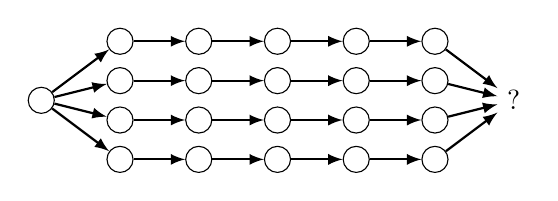
\begin{tikzpicture}
      \node[git/commit] (c0) at (0,0) {};
      \node (end) at (6,0) { ? };

      \foreach[count=\i] \y in {-0.25,-0.75,0.25,0.75} {
        \foreach \x in {1,...,5} {
          \node[git/commit] (c\i-\x) at (\x,\y) {};
        }
        \foreach[evaluate={int(\x-1)} as \z] \x in {2,...,5} {
          \draw[git/commit arrow] (c\i-\z) -- (c\i-\x);
        }
        \draw[git/commit arrow] (c0) -- (c\i-1);
        \draw[git/commit arrow] (c\i-5) -- (end);
      }
    \end{tikzpicture}
  \end{center}
\end{frame}

\begin{frame}
  \frametitle{Manual Solution}
  \begin{center}
    \begin{tikzpicture}
      \path[use as bounding box] (0,0) rectangle ++(6,-5.5);

      \only<1-2>{
        \directory[id=root,position={(0,0)}]{project}
        \directory[id=trunk,subdirectory of=root distance 1]{trunk}
        \directory[id=tb1,subdirectory of=trunk distance 1]{20220329-1531}
        \directory[id=tb2,subdirectory of=trunk distance 2]{20220330-1022}
        \directory[id=tb3,subdirectory of=trunk distance 3]{20220330-1357}

        \directory[id=feature a,subdirectory of=root distance 5]{feature-a}
        \directory[id=a working area,subdirectory of=feature a distance 1]{working-area}
        \directory[id=a backups,subdirectory of=feature a distance 2]{backups}
        \directory[id=a backups 1,subdirectory of=a backups distance 1]{20220331-1403}
        \directory[id=a backups 2,subdirectory of=a backups distance 2]{20220331-1512}
        \directory[id=a backups 3,subdirectory of=a backups distance 3]{20220331-1544}
        \directory[id=a backups 4,subdirectory of=a backups distance 4]{20220401-1024}

        \draw[fs/dirlink] (root) |- (trunk);
        \draw[fs/dirlink] (trunk) |- (tb1);
        \draw[fs/dirlink] (trunk) |- (tb2);
        \draw[fs/dirlink] (trunk) |- (tb3);

        \draw[fs/dirlink] (root) |- (feature a);
        \draw[fs/dirlink] (feature a) |- (a working area);
        \draw[fs/dirlink] (feature a) |- (a backups);
        \draw[fs/dirlink] (a backups) |- (a backups 1);
        \draw[fs/dirlink] (a backups) |- (a backups 2);
        \draw[fs/dirlink] (a backups) |- (a backups 3);
        \draw[fs/dirlink] (a backups) |- (a backups 4);
      }

      \only<3->{
        \directory[id=root,position={(0,0)}]{project}
        \directory[id=trunk,subdirectory of=root distance 1]{trunk}
        \directory[id=tb1,subdirectory of=trunk distance 1]{20220329-1531}
        \directory[id=tb2,subdirectory of=trunk distance 2]{20220330-1022}
        \directory[id=tb3,subdirectory of=trunk distance 3]{20220330-1357}
        \directory[id=a backups 1,subdirectory of=trunk distance 4]{20220331-1403}
        \directory[id=a backups 2,subdirectory of=trunk distance 5]{20220331-1512}
        \directory[id=a backups 3,subdirectory of=trunk distance 6]{20220331-1544}
        \directory[id=a backups 4,subdirectory of=trunk distance 7]{20220401-1024}

        \draw[fs/dirlink] (root) |- (trunk);
        \draw[fs/dirlink] (trunk) |- (tb1);
        \draw[fs/dirlink] (trunk) |- (tb2);
        \draw[fs/dirlink] (trunk) |- (tb3);
        \draw[fs/dirlink] (trunk) |- (a backups 1);
        \draw[fs/dirlink] (trunk) |- (a backups 2);
        \draw[fs/dirlink] (trunk) |- (a backups 3);
        \draw[fs/dirlink] (trunk) |- (a backups 4);
      }

      \only<1>{
        \draw[comment line,latex-] (a backups 4-node.east) -| ++(2.5,1) node[comment box,anchor=south] (comment) {\parbox{4cm}{Feature a has been finalized}};
      }

      \only<2>{
        \node[comment box,anchor=west] at ($ (trunk-node.east) + (3,0) $) {\parbox{4cm}{Finished features should be incorporated into the trunk}};

        \foreach \i in {1,2,3,4} {
          \draw[move arrow] (a backups \i-node.east) -- ++(0.5,0) |- (trunk-node.east);
        }
      }
    \end{tikzpicture}
  \end{center}
  \begin{overprint}
    \onslide<2>
    \begin{center}
      
\begin{tikzpicture}
        \node[console] {
          \$ mv feature-a/backups/* trunk
        };
      \end{tikzpicture}
    \end{center}
  \end{overprint}
\end{frame}

\begin{frame}
  \frametitle{Merging}
  \begin{center}
    \begin{tikzpicture}
      \node[git/commit] (master 1) at (0,0) {};
      \node[git/commit] (master 2) at ($ (master 1) + (1,0) $) {};
      \node[git/commit] (master 3) at ($ (master 2) + (1,0) $) {};
      \node[git/commit] (feature 1) at ($ (master 3) + (1,1) $) {};
      \node[git/commit] (feature 2) at ($ (feature 1) + (1,0) $) {};
      \node[git/commit] (feature 3) at ($ (feature 2) + (1,0) $) {};
      \node[git/commit] (feature 4) at ($ (feature 3) + (1,0) $) {};

      \visible<2>{
        \node[git/commit] (merged) at ($ (feature 4) + (1,-1) $) {};
      }

      \foreach \x/\y in {master 1/master 2,master 2/master 3,master 3/feature 1,feature 1/feature 2,feature 2/feature 3,feature 3/feature 4} {
        \draw[git/commit arrow] (\x) -- (\y);
      }

      \visible<1>{
        \draw[latex-] (master 3) -- ++(0,-1) node[git/ref] (master) {\master};
      }
      \visible<2->{
        \draw[latex-] (merged) -- ++(0,-1) node[git/ref] (master merged) {\master};
      }

      \draw[latex-] (feature 4) -- ++(0,1) node[git/ref] (master) {feature};

      \visible<2>{
        \draw[git/commit arrow] (master 3) -- (merged);
        \draw[git/commit arrow] (feature 4) -- (merged);
      }

      \only<1>{
        \begin{scope}[overlay]
          \draw[latex-,comment line] (feature 4) -- ++(0,-1) node[comment box,anchor=north] {Fully developed feature};
        \end{scope}
      }

      \only<2>{
        \begin{scope}[overlay]
          \draw[latex-,comment line] (master merged) -- ++(-1,0) node[comment box,anchor=east] {\parbox{5cm}{A new commit is made to join \texttt{\master} and \texttt{feature} {\tiny (white lie)}}};
        \end{scope}
      }
    \end{tikzpicture}
  \end{center}
  \vskip5mm
  \begin{overprint}
    \onslide<2>
    \begin{center}
      
\begin{tikzpicture}
        \node[console] {
          \parbox{4cm}{
            \$ git checkout master \\
            \$ git merge feature
          }
        };
      \end{tikzpicture}
    \end{center}
  \end{overprint}
\end{frame}

\begin{frame}
  \frametitle{Problem Statement}
  \begin{itemize}
    \item Example situation was very easy to deal with
    \item The \texttt{feature} branch is an extension of \texttt{\master}
    \item Merging consists of simply copying from \texttt{feature} to \texttt{\master}
    \item But it's not always this simple\dots
  \end{itemize}
\end{frame}

\begin{frame}
  \frametitle{Multiple Branches}
  \begin{center}
    \begin{tikzpicture}
      \node[git/commit] (master 1) at (0,0) {};
      \node[git/commit] (master 2) at ($ (master 1) + (1,0) $) {};
      \node[git/commit] (master 3) at ($ (master 2) + (1,0) $) {};
      \node[git/commit] (feature a 1) at ($ (master 3) + (1,1) $) {};
      \node[git/commit] (feature a 2) at ($ (feature a 1) + (1,0) $) {};
      \node[git/commit] (feature a 3) at ($ (feature a 2) + (1,0) $) {};
      \node[git/commit] (feature b 1) at ($ (master 3) + (1,-1) $) {};
      \node[git/commit] (feature b 2) at ($ (feature b 1) + (1,0) $) {};
      \node[git/commit] (feature b 3) at ($ (feature b 2) + (1,0) $) {};
      \node[git/commit] (feature b 4) at ($ (feature b 3) + (1,0) $) {};
      \node[git/commit] (feature b 5) at ($ (feature b 4) + (1,0) $) {};
      \node[git/commit] (master a merge) at ($ (feature a 3) + (1,-1) $) {};
      \visible<3->{
        \node (master b merge) at ($ (feature b 5) + (1,1) $) {?};
      }

      \foreach \x/\y in {master 1/master 2,master 2/master 3,master 3/feature a 1,feature a 1/feature a 2,feature a 2/feature a 3,feature a 3/master a merge,master 3/feature b 1,feature b 1/feature b 2,feature b 2/feature b 3,feature b 3/feature b 4,feature b 4/feature b 5,master 3/master a merge} {
        \draw[git/commit arrow] (\x) -- (\y);
      }

      \visible<3->{
        \foreach \x/\y in {master a merge/master b merge,feature b 5/master b merge} {
          \draw[git/commit arrow] (\x) -- (\y);
        }
      }

      \draw[latex-] (master a merge) -- ++(0,0.5) node[git/ref,anchor=south] (master) { \master };
      \draw[latex-] (feature a 3) -- ++(0,0.5) node[git/ref,anchor=south] (feature a) { feature-a };
      \draw[latex-] (feature b 5) -- ++(0,-0.5) node[git/ref,anchor=north] (feature b) { feature-b };

      \only<1>{
        \begin{scope}[overlay]
          \draw[latex-,comment line] (feature b) -- ++(0,-0.5) node[comment box,anchor=north] {\parbox{5cm}{Developed separately in parallel with feature A}};
        \end{scope}
      }

      \only<2>{
        \begin{scope}[overlay]
          \node[comment box,anchor=east] at ($ (feature b) + (-1,-1) $) {\parbox{5cm}{We cannot just copy feature B over \master: we would lose feature A}};
        \end{scope}
      }

      \only<3>{
        \begin{scope}[overlay]
          \draw[latex-,comment line] (master b merge) -- ++(0,1) node[comment box,anchor=south] {\parbox{4cm}{Some Git magic needs to happen here}};
        \end{scope}
      }
    \end{tikzpicture}
  \end{center}
\end{frame}

\begin{frame}
  \frametitle{Merging: Separate Files}
  \begin{center}
    \begin{tikzpicture}
      \node[git/commit] (master) at (0,0) {};
      \node[git/commit] (feature a) at ($ (master) + (1,1) $) {};
      \node[git/commit] (feature b) at ($ (master) + (1,-1) $) {};
      \node (merge) at ($ (feature a) + (1,-1) $) {?};

      \foreach \x/\y in {master/feature a,master/feature b,feature a/merge,feature b/merge,master/merge} {
        \draw[git/commit arrow] (\x) -- (\y);
      }

      \draw[latex-] (master) -- ++(-0.5,0) node[git/ref,anchor=east] (master ref) {\master};
      \draw[latex-] (feature a) -- ++(0,0.5) node[git/ref,anchor=south] (a ref) {feature-a};
      \draw[latex-] (feature b) -- ++(0,-0.5) node[git/ref,anchor=north] (b ref) {feature-b};

      \only<1>{
        \begin{scope}[overlay]
          \draw[comment line,latex-] (a ref) -- ++(0,0.5) node[comment box,anchor=south] {Added file \texttt{a.py}};
          \draw[comment line,latex-] (b ref) -- ++(0,-0.5) node[comment box,anchor=north] {Added file \texttt{b.py}};
        \end{scope}
      }

      \only<2>{
        \begin{scope}[overlay]
          \draw[comment line,latex-] (merge) -- ++(0,1) node[comment box,anchor=south] {Simply add both \texttt{a.py} and \texttt{b.py}};
        \end{scope}
      }
    \end{tikzpicture}
  \end{center}
\end{frame}

\begin{frame}
  \frametitle{Merging: Branches Modify Same File}
  \begin{center}
    \begin{tikzpicture}
      \node[git/commit] (master) at (0,0) {};
      \node[git/commit] (feature a) at ($ (master) + (1,1) $) {};
      \node[git/commit] (feature b) at ($ (master) + (1,-1) $) {};
      \node (merge) at ($ (feature a) + (1,-1) $) {?};

      \foreach \x/\y in {master/feature a,master/feature b,feature a/merge,feature b/merge,master/merge} {
        \draw[git/commit arrow] (\x) -- (\y);
      }

      \draw[latex-] (master) -- ++(-0.5,0) node[git/ref,anchor=east] (master ref) {\master};
      \draw[latex-] (feature a) -- ++(0,0.5) node[git/ref,anchor=south] (a ref) {feature-a};
      \draw[latex-] (feature b) -- ++(0,-0.5) node[git/ref,anchor=north] (b ref) {feature-b};

      \only<1>{
        \begin{scope}[overlay]
          \draw[comment line,latex-] (a ref) -- ++(0,0.5) node[comment box,anchor=south] {Updated file \texttt{app.py}};
          \draw[comment line,latex-] (b ref) -- ++(0,-0.5) node[comment box,anchor=north] {Updated file \texttt{app.py}};
        \end{scope}
      }

      \only<2>{
        \begin{scope}[overlay]
          \draw[comment line,latex-] (merge) -- ++(0,1) node[comment box,anchor=south] {Must somehow merge changes to \texttt{app.py}};
        \end{scope}
      }
    \end{tikzpicture}
  \end{center}
\end{frame}

\begin{frame}
  \frametitle{Merge Files}
  \begin{center}
    \begin{tikzpicture}
      \foreach[count=\i] \y in {0,-0.2,...,-5} {
        \coordinate (left line \i) at (0,\y);
        \coordinate (middle line \i) at (4,\y);
        \coordinate (right line \i) at (8,\y);
      }

      \foreach[evaluate={(\i-1)*-0.2} as \y] \i in {1,2,9,10,...,26} {
        \codeline[x=0,y=\y]
      }

      \foreach[evaluate={(\i-1)*-0.2} as \y] \i in {3,...,8} {
        \codeline[x=0,y=\y,color=red]
      }

      \foreach[evaluate={(\i-1)*-0.2} as \y] \i in {1,...,16,24,25,26} {
        \codeline[x=8,y=\y]
      }

      \foreach[evaluate={(\i-1)*-0.2} as \y] \i in {17,...,23} {
        \codeline[x=8,y=\y,color=green]
      }

      \coordinate (top left) at (left line 1);
      \coordinate (bottom left) at (left line 26);
      \coordinate (middle left) at ($ (top left) ! 0.5 ! (bottom left) $);

      \coordinate (top right) at (right line 1);
      \coordinate (bottom right) at (right line 26);
      \coordinate (middle right) at ($ (top right) ! 0.5 ! (bottom right) $);

      \node[anchor=south west,minimum width=3cm] at (0,0.25) {\texttt{feature-a}};
      \node[anchor=south west,minimum width=3cm] at (4,0.25) {merged result};
      \node[anchor=south west,minimum width=3cm] at (8,0.25) {\texttt{feature-b}};

      \only<1>{
        \draw[|-|] ($ (left line 1) + (3.5,0) $) -- ($ (left line 26) + (3.5, 0) $);
        \draw[|-|] ($ (right line 1) + (-0.5,0) $) -- ($ (right line 26) + (-0.5, 0) $);
        \draw[latex-,comment line] ($ (top left) ! 0.33 ! (bottom left) + (3.5,0) $) -- ++(0.5,0) node[comment box,anchor=west] {\parbox{3cm}{\texttt{app.py} according to \texttt{feature-a}}};
        \draw[latex-,comment line] ($ (top right) ! 0.66 ! (bottom right) + (-0.5,0) $) -- ++(-0.5,0) node[comment box,anchor=east] {\parbox{3cm}{\texttt{app.py} according to \texttt{feature-b}}};
      }

      \only<2>{
        \begin{scope}[overlay]
          \draw[opacity=0.25,fill=red] ($ (left line 3) + (-0.1,0.1) $) rectangle ($ (left line 8) + (3.5,-0.1) $);
          \draw[opacity=0.25,fill=red] ($ (right line 17) + (-0.1,0.1) $) rectangle ($ (right line 23) + (3.5,-0.1) $);
          \draw[latex-,comment line] ($ (left line 3) ! 0.5 ! (left line 8) + (3.5,0) $) -- ++(0.5,0) node[comment box,anchor=west] {\parbox{3.25cm}{Modifications made by \texttt{feature-a}}};
          \draw[latex-,comment line] ($ (right line 17) ! 0.5 ! (right line 23) + (-0.1,0) $) -- ++(-0.5,0) node[comment box,anchor=east] {\parbox{3.25cm}{Modifications made by \texttt{feature-b}}};
        \end{scope}
      }

      \only<3->{
        \foreach[evaluate={(\i-1)*-0.2} as \y] \i in {1,2,9,10,...,16,24,25,26} {
          \codeline[x=4,y=\y]
        }
      }

      \only<3>{
        \begin{scope}[overlay]
          \node[comment box,anchor=south west] at ($ (left line 25) + (0.1,0.1) $) { \parbox{4cm}{Unchanged parts can be preserved in merged result} };
        \end{scope}
      }

      \only<4->{
        \foreach[evaluate={(\i-1)*-0.2} as \y] \i in {3,...,8} {
        \codeline[x=4,y=\y,color=red]
        }

        \foreach[evaluate={(\i-1)*-0.2} as \y] \i in {17,...,23} {
          \codeline[x=4,y=\y,color=green]
        }
      }

      \only<4>{
        \begin{scope}[overlay]
          \node[comment box,anchor=north west] at ($ (middle line 10) + (-1.1,0.1) $) { \parbox{4cm}{Changes make it into to merged result} };
          \coordinate (left start) at ($ (left line 3) + (2,0) $);
          \coordinate (left end) at ($ (left line 8) + (2,0) $);
          \coordinate (left middle) at ($ (left start) ! 0.5 ! (left end) $);
          \coordinate (lmiddle start) at ($ (middle line 3) + (-0.2,0) $);
          \coordinate (lmiddle end) at ($ (middle line 8) + (-0.2,0) $);
          \coordinate (lmiddle middle) at ($ (lmiddle start) ! 0.5 ! (lmiddle end) $);

          \coordinate (right start) at ($ (right line 17) + (-0.2,0) $);
          \coordinate (right end) at ($ (right line 23) + (-0.2,0) $);
          \coordinate (right middle) at ($ (right start) ! 0.5 ! (right end) $);
          \coordinate (rmiddle start) at ($ (middle line 17) + (3.3,0) $);
          \coordinate (rmiddle end) at ($ (middle line 23) + (3.3,0) $);
          \coordinate (rmiddle middle) at ($ (rmiddle start) ! 0.5 ! (rmiddle end) $);

          \draw[|-|] (left start) -- (left end);
          \draw[|-|] (lmiddle start) -- (lmiddle end);
          \draw[-latex,thick] (left middle) -- (lmiddle middle);

          \draw[|-|] (right start) -- (right end);
          \draw[|-|] (rmiddle start) -- (rmiddle end);
          \draw[-latex,thick] (right middle) -- (rmiddle middle);
        \end{scope}
      }
    \end{tikzpicture}
  \end{center}
\end{frame}

\begin{frame}
  \frametitle{Merge Conflicts}
  \begin{center}
    \begin{tikzpicture}
      \foreach[count=\i] \y in {0,-0.2,...,-5} {
        \coordinate (left line \i) at (0,\y);
        \coordinate (middle line \i) at (4,\y);
        \coordinate (right line \i) at (8,\y);
      }

      \foreach[evaluate={(\i-1)*-0.2} as \y] \i in {1,2,...,9,17,18,...,26} {
        \codeline[x=0,y=\y]
      }

      \foreach[evaluate={(\i-1)*-0.2} as \y] \i in {10,...,16} {
        \codeline[x=0,y=\y,color=red]
      }

      \foreach[evaluate={(\i-1)*-0.2} as \y] \i in {1,...,12,20,21,...,26} {
        \codeline[x=8,y=\y]
      }

      \foreach[evaluate={(\i-1)*-0.2} as \y] \i in {13,...,19} {
        \codeline[x=8,y=\y,color=green]
      }

      \coordinate (top left) at (left line 1);
      \coordinate (bottom left) at (left line 26);
      \coordinate (middle left) at ($ (top left) ! 0.5 ! (bottom left) $);

      \coordinate (top right) at (right line 1);
      \coordinate (bottom right) at (right line 26);
      \coordinate (middle right) at ($ (top right) ! 0.5 ! (bottom right) $);

      \node[anchor=south west,minimum width=3cm] at (0,0.25) {\texttt{feature-a}};
      \node[anchor=south west,minimum width=3cm] at (4,0.25) {merged result};
      \node[anchor=south west,minimum width=3cm] at (8,0.25) {\texttt{feature-b}};

      \only<1>{
        \begin{scope}[overlay]
          \node[comment box,anchor=south west] at ($ (left line 25) + (0.1,0.1) $) { \parbox{6cm}{Consider the case where \texttt{feature-a} and \texttt{feature-b} updated the overlapping pieces of code} };
        \end{scope}
      }

      \only<2->{
        \foreach[evaluate={(\i-1)*-0.2} as \y] \i in {1,...,9,20,21,...,26} {
          \codeline[x=4,y=\y]
        }
      }

      \only<2>{
        \begin{scope}[overlay]
          \node[comment box,anchor=south west] at ($ (left line 25) + (0.1,0.1) $) { \parbox{4cm}{Unchanged parts can again be preserved} };
        \end{scope}
      }

      \only<3->{
        \node at ($ (middle line 15) + (1,0) $) (conflict) {\Huge ?};
        \node[comment box,anchor=south west] at ($ (left line 25) + (0.1,-0.5) $) { \parbox{6cm}{However, Git cannot possibly guess how to merge the overlapping changes} };
        \draw[latex-,comment line] (conflict) -- ++(0,1) node[comment box,anchor=south] {Merge conflict};
      }
    \end{tikzpicture}
  \end{center}
\end{frame}

% IGNORE

\section{.gitignore}

\begin{frame}
  \tableofcontents[currentsection]
\end{frame}

\begin{frame}
  \frametitle{Files}
  \begin{itemize}
    \item Not all files should be \texttt{add}ed to the repository
    \item Only source files!
    \item "Generatable" files should not be added
  \end{itemize}
\end{frame}

\begin{frame}
  \frametitle{Java Example}
  \begin{center}
    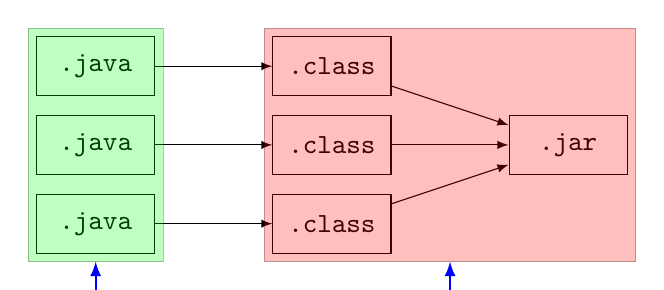
\begin{tikzpicture}[file/.style={font=\ttfamily,minimum width=1.5cm,minimum height=.75cm,draw}]
      \node[file] (java 1) { .java };
      \node[file] (java 2) at ($ (java 1) + (0,1) $) { .java };
      \node[file] (java 3) at ($ (java 2) + (0,1) $) { .java };

      \foreach \i in {1,2,3} {
        \node[file] (class \i) at ($ (java \i) + (3,0) $) { .class };
        \draw[-latex] (java \i) -- (class \i);
      }

      \node[file] (jar) at ($ (class 2) + (3,0) $) { .jar };
      \foreach \i in {1,2,3} {
        \draw[-latex] (class \i) -- (jar);
      }

      \draw[opacity=.25,fill=green] ($ (java 1.south west) + (-0.1,-0.1) $) rectangle ($ (java 3.north east) + (0.1,0.1) $);
      \draw[opacity=.25,fill=red] let \p1=(class 1.south west), \p2=(class 3.north), \p3=(jar.east) in ($ (class 1.south west) + (-0.1,-0.1) $) coordinate (p1) rectangle ($ (\x3,\y2) + (0.1,0.1) $) coordinate (p2);

      \coordinate (anchor 1) at ($ (java 1.south) + (0,-0.1) $);
      \path let \p1=(p1), \p2=(p2) in ($ (\x1,\y1) ! 0.5 ! (\x2,\y1) $) coordinate (anchor 2);

      \draw[latex-,comment line] (anchor 1) -- ++(0,-0.5) node[comment box,anchor=north] { add };
      \draw[latex-,comment line] (anchor 2) -- ++(0,-0.5) node[comment box,anchor=north] { don't add };
    \end{tikzpicture}
  \end{center}
\end{frame}

\begin{frame}
  \frametitle{Binary Files}
  \begin{itemize}
    \item Files in binary form instead of text form
          \begin{itemize}
            \item Images (png, jpeg, \dots)
            \item Audio (wav, mp3, ogg, midi, \dots)
            \item Compressed files (zip, 7z, \dots)
          \end{itemize}
    \item Typically large
    \item {\color{red} Do not add them to the repository}
    \item Be careful! Once added, it's very hard to remove them!
    \item Share such files manually (e.g., using OneDrive)
  \end{itemize}
\end{frame}

\begin{frame}
  \frametitle{How to Not Add Files}
  \begin{itemize}
    \item Do not \texttt{git add} them
    \item List forbidden files in \texttt{.gitignore}
  \end{itemize}
  \vskip5mm
  \begin{center}
    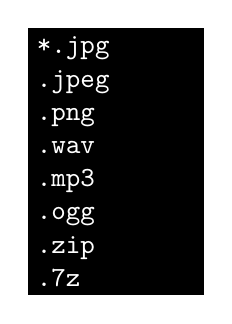
\begin{tikzpicture}
      \node[fill=black,text=white,font=\ttfamily]{
        \parbox{2cm}{
          *.jpg \\
          *.jpeg \\
          *.png \\
          *.wav \\
          *.mp3 \\
          *.ogg \\
          *.zip \\
          *.7z
        }
      };
    \end{tikzpicture}
  \end{center}
\end{frame}

\end{document}
